Для последнего задания возьмем логотип немецкого производителя автомобилей -- \textbf{BMW}.

\begin{figure}[ht!]
    \centering
    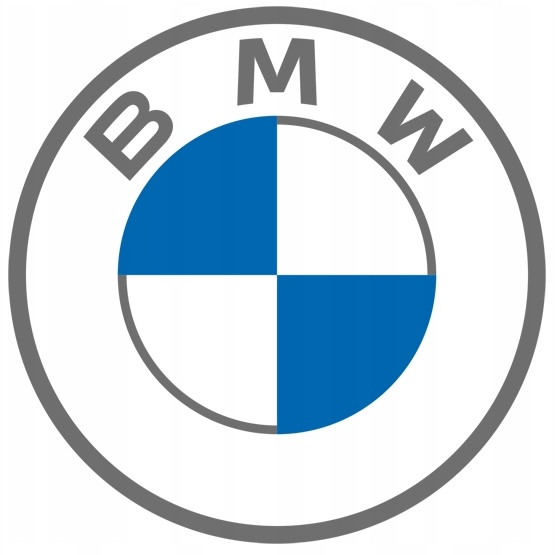
\includegraphics[width=0.5\textwidth]{images/source_images/task_4/bmw.jpeg}
    \caption{Логотип компании \textbf{BMW AG}}
    \label{fig:bmw}
\end{figure}
Для выделения контуров на изображении возьмём матрицу.
\begin{gather}
    K = \begin{pmatrix}
        -1 & -1 & -1\\
        -1 & 8 & 1-\\
        -1 & -1 & -1
    \end{pmatrix}  
\end{gather}

Применим её на изображение посредством свёртки и Фурье-преобразований:

\begin{figure}[ht!]
    \centering
    
\includegraphics[width=0.6\textwidth]{images/result/task_4/Edges.png}
    \caption{Контуры изображения, полученные при использовании свертки}
    \label{fig:ed_c}
\end{figure}

\begin{figure}[ht!]
    \centering
    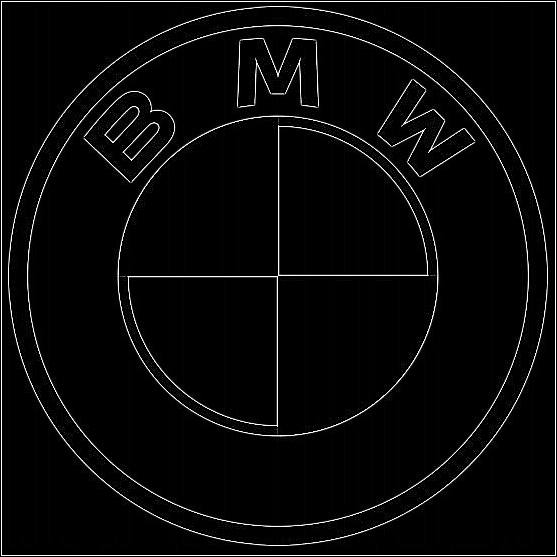
\includegraphics[width=0.6\textwidth]{images/result/task_4/Edges_fourier.png}
    \caption{Контуры изображения, полученные при использовании преобразований Фурье}
    \label{fig:ed_f}
\end{figure}

И снова мы получили одинаковые изображения (без учёта границы на изображении, полученном при использовании преобразований Фурье. Объяснение приведено в заключительном абзаце прошлого пункта).

Код программ для выполнения этой лабораторной работы и полученные изображения находятся в репозитории (\href{https://github.com/NikBrat/Lab_6_CM}{ссылка}).